%!TEX root = thesis.tex

\chapter{Implementation}
\label{chap:impl}

Implementation of the methods are described in this chapter.

\section{Preparing linked data}
Linked data has been prepared that is used to retrieve and process sensor data on the semantic web (Figure \ref*{fig:Static}). This is done for vector data sets of administrative units and land cover features, and for raster data sets of \ac{eea} grids with a resolution of 10km\textsuperscript{2} and 100km\textsuperscript{2}. 

\begin{figure}
	%\centering
	\includegraphics[width=0.7\linewidth]{UML/staticdata2.PNG}
	\caption{Model of vector and raster features}
	\label{fig:Static}
\end{figure}


Three types of administrative units have been converted to linked data: countries, provinces and municipalities. Every administrative unit has a name, `type' and (multi)polygon geometry assigned to it (Figure \ref{fig:Static}). The administrative unit type is defined by DBPedia \ac{uri}s of country, province and municipality. 

The \ac{corine} 2012 land cover dataset contains features with an identifier, a land cover type and a (multi)polygon geometry (Figure \ref{fig:Static}). The identifier has the form of: `EU-' plus a unique seven digit number. The land cover type is defined by a three digit number, which can looked up in the provided spreadsheet containing the legend.    

The \ac{eea} reference grid with resolutions of 10km\textsuperscript{2} and 100km\textsuperscript{2}. Every feature is defined by an identifier, a resolution and a point geometry of the origin (Figure \ref{fig:Static}). The identifier is a code given to a feature by the \ac{eea} and has the form of: resolution + `E' + x coordinate + `N' + y coordinate.   

\section{Publishing linked data}
Setting up the Strabon (Figure \ref{fig:Strabon}), Apache Tomcat and Pubby software. 

The Strabon and Parliament endpoint have been tested since they both handle GeoSPARQL queries. Strabon has been used in the final implementation, because the Parliament endpoint rejected certain longer queries (see \ref{par:spQueries}). \\

Pubby software in combination with Apache Tomcat allows for a user interface that is easier to navigate through for humans. The links stored in \ac{rdf} triples are represented as hyperlinks which can be used to navigate between pages about different concepts. \\

For creating \aclp{purl} the Purlz software (\url{http://www.purlz.org/}) has been used. All \acp{uri} that are created get a \ac{purl} assigned to it. The \ac{purl} resolves the \ac{uri} to a \texttt{DESCRIBE} query at the endpoint. This query is structured as a get request: \texttt{\seqsplit{http://localhost/strabon-endpoint-3.3.2-SNAPSHOT/Describe?submit=describe\&view=HTML\&handle=download\&format=turtle\&query=DESCRIBE < an\_URI >}}. The request has `\texttt{/Describe?submit=describe}' to call the script that deals with describe queries and to tell it that the request is also submitting this kind of query. The parameters `\texttt{view=HTML\&handle=download}' indicate that the endpoint's website is requested, but the returned data should be a download file instead of an HTML page. The parameter `\texttt{\&format=turtle}' sets the \ac{rdf} notation of the download file to Turtle and `\texttt{\&query=DESCRIBE <an\_URI>}' is the \ac{sparql} query that contains the \ac{uri} between brackets. 

Every \ac{uri} is written to an \ac{xml} file with the parameters: ID, \ac{purl} type, and target address. Optionally, information about the person or organisation maintaining the \ac{purl} can be added. The ID is the original \ac{uri} that is being resolved to the target address. The \ac{purl} type is set to 303, which means that it refers the client to the target address. Alternative types can be found in Table \ref{tbl:HTTP}. After all \acp{uri} have been added to the so called \ac{xml} `batch' file \citep{LD:PURL2}, the file can be posted to the Purlz server. \\

\begin{table}[]
	\centering
	\caption{Types of PURLs \citep{LD:PURL}}
	\label{tbl:HTTP}
	\resizebox{\textwidth}{!}{%
	\begin{tabular}{lll}
		PURL Type & Meaning                                         & HTTP Shorthand     \\
		301       & Moved permanently to a target \ac{url}          & Moved Permanently  \\
		302       & Simple redirection to a target \ac{url}         & Found              \\
		303       & See other \acp{url} (use for Semantic Web resources) & See Other     \\
		307       & Temporary redirect to a target \ac{url}         & Temporary Redirect \\
		404       & Temporarily gone                                & Not Found          \\
		410       & Permanently gone                                & Gone              
	\end{tabular}
}
\end{table}

Setting it up on the university server

\begin{figure}
	\centering
	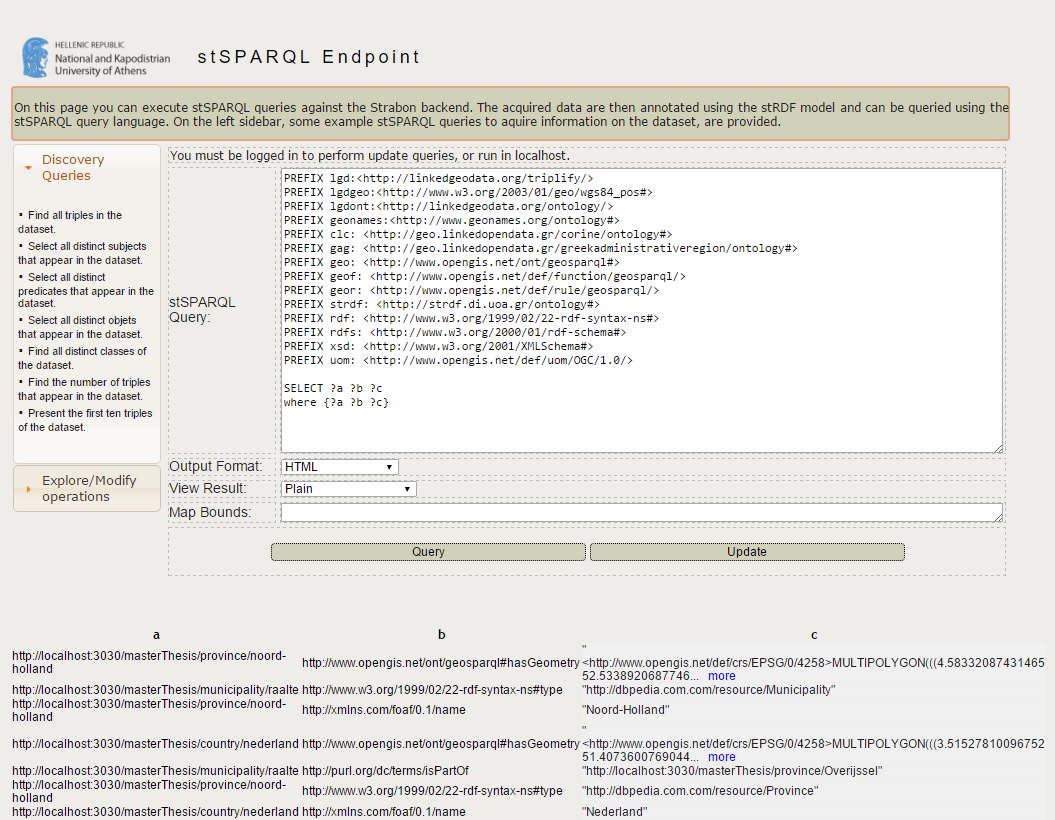
\includegraphics[width=\linewidth]{figs/Strabon.PNG}
	\caption{Strabon endpoint}
	\label{fig:Strabon}
\end{figure}

%\begin{figure}
	%\centering
%	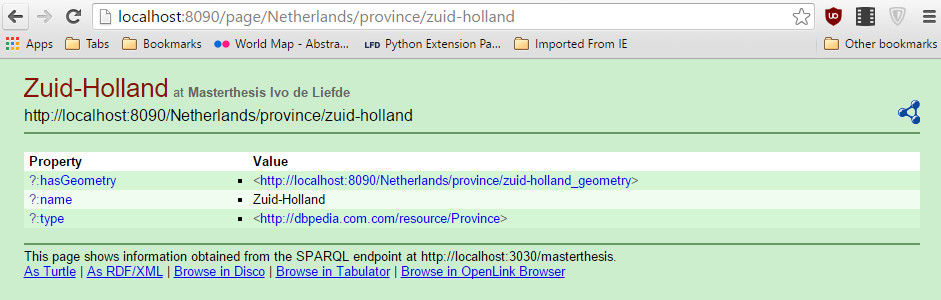
\includegraphics[width=\linewidth]{figs/pubby.PNG}
%	\caption{Pubby interface for \ac{rdf}}
%	\label{fig:Pubby}
%\end{figure}


\section{Retrieving metadata from the Sensor Observation Service}
The metadata is automatically retrieved from the \ac{sos} according to Figure \ref{fig:SOS_UML}. A \ac{sos} is maintained by an organisation, of which the name is retrieved, as well as whether they charge fees or have implemented access constraints for using the \ac{sos}. In most cases the use is free of charge and without access constraints. However, it is possible for an organisation to restrict the use of the \ac{sos} in these ways. 

In the \ac{swe} standards a sensor is modelled using two entities: a procedure and a feature of interest. The procedure is the method of sensing and the feature of interest is the feature of which the sensor is sensing a certain property. Therefore, the observable property ties together the procedure and feature of interest. It should be noted that the geometry of a feature of interest is not necessarily always a point geometry. It can also be generalized into larger features (e.g. multiple sensors observing different parts of one lake). 

An offering is a grouping of features of interest, which have a common procedure. The purpose of offerings is to allow users to query the observation data more efficiently. Features of interest that are often queried together are grouped into the same offering.      
 

\begin{figure}
	\centering
	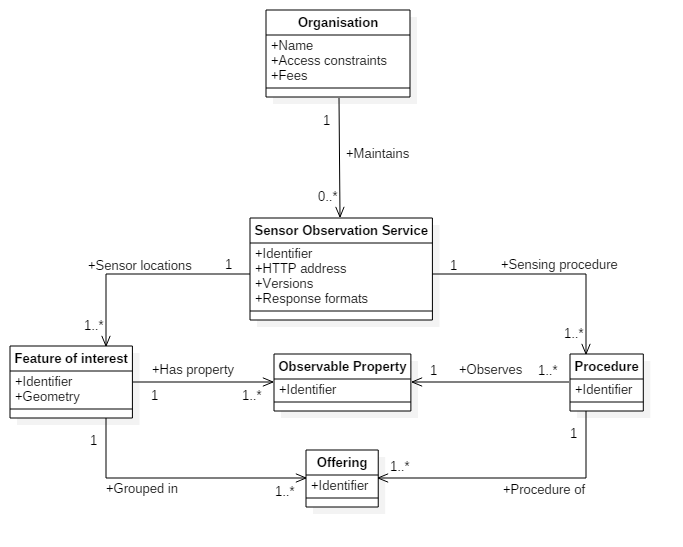
\includegraphics[width=\linewidth]{UML/SOS_UML.PNG}
	\caption{Metadata automatically retrieved from a \ac{sos}}
	\label{fig:SOS_UML}
\end{figure}

A Python class object is created for the \ac{sos} based on Figure \ref{fig:SOS_UML}. This class contains the different variables and has built in functions to automatically retrieve the metadata. To collect all the required metadata a number of request have to be made, which is done using the \texttt{SOSclass.request()} method which requires only the \ac{http} address of the \ac{sos} as input. First, the capabilities document is retrieved to collect information about the organisation, supported \ac{sos} versions and response formats. It also contains lists with identifiers for all features of interest, offerings, observable properties and procedures. In this document the offerings are linked to a certain procedure and to a certain observable property. 

Unfortunately, the capabilities document is not able to provide information about which procedure is being applied for which feature of interest. Also, the features' geometries cannot be retrieved from it. Therefore, a \texttt{GetFeatureOfInterest} request is made to retrieve the location of each features of interest. However, the \texttt{GetFeatureOfInterest} document does not necessarily provide information about the procedures that are related to a certain feature of interest. When a \texttt{GetObservation} request is made for an offering, the returned observation data is grouped per feature of interest. 
Therefore, small amounts of data are retrieved from each offering using \texttt{GetObservation} requests, when possible with a temporal filter to limit the data traffic. 
Every procedure and offering can now be related to a set of features of interest with point geometries.  
 

\section{Modelling with the om-lite and sam-lite ontologies}
\begin{figure}
	\centering
	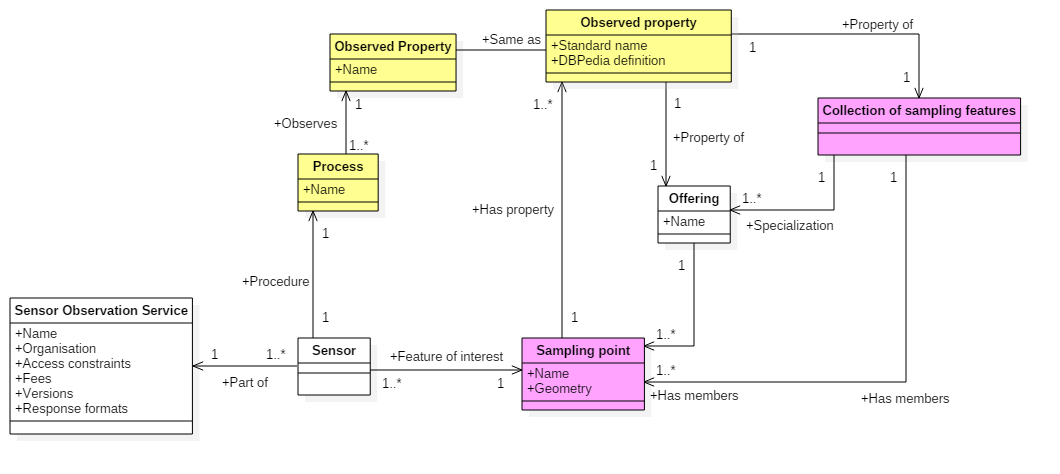
\includegraphics[width=1\linewidth]{UML/SOS_Semantic_UML.PNG}
	\caption{Sensor metadata as modelled in RDF (om-lite classes in yellow and sam-lite classes in purple)}
	\label{fig:SOS_Semantic_UML}
\end{figure}

After the metadata has been retrieved from the \ac{sos} (Figure \ref{fig:SOS_UML}) it has to be converted to linked data. For this the om-lite and sam-lite ontologies are being used in combination with the PROV and GeoSPARQL ontologies. Figure \ref{fig:SOS_Semantic_UML} shows the semantic relations between the metadata that are stored in \ac{rdf} triples. Every (instance of a) class in this figure is represented by a \ac{uri}. 

A \ac{sos} is modelled as an agent with a specific name, that acts on behalf of a certain organisation. The organisation, access constraints, fees, versions and response formats are properties of the \ac{sos}. Every sensor is described by a procedure and a certain feature of interest. The sensor class was not present in the model of Figure \ref{fig:SOS_UML}, because the \ac{sos} does not define sensors. However, the sensor class has been added to the semantic model to make the relation between procedure and sampling point explicit. 

In Figure \ref{fig:SOS_Semantic_UML} the collection of sampling features only contains sampling points. This is because the feature of interest of an air quality sensor is equal to the bubble of air directly around the sampling point. Other sampling features can be added when the application requires this. Sampling features are grouped into collections of features of which the same observed property is measured. These collections can contain sampling points from multiple \aclp{sos}. The offering class is a specialization of the collection of sampling features. It contains a subset of the sampling points that are all part of the same offering at a particular \ac{sos}.

Every observed property that is defined in a \ac{sos} relates to a certain observed property as defined by DBPedia. Since \ac{sos} requests require their own identifiers as input the observed property class exists twice in the model: one as defined by the \ac{sos} and one as defined by DBPedia. For the same reason all sampling points, processes and offerings have a `name' attribute in addition to their \ac{uri}. These store the original identifier that they were given by the \ac{sos}.

\section{Establishing inward links from DBPedia}
Sending triples to DBPedia the project to be uploaded.

Contains links from DBPedia page of `\acl{sos}' to the semantic definition of the input \ac{sos}, from the DBPedia page of `ozone', `particulate matter' and `nitrogen dioxide' to the corresponding collections of sampling features.

Also, the data of administrative units, land cover features and \ac{eea} reference grid cells will be linked to from DBPedia.

\section{Prototype implementation}
The prototype implementation serves as a proof of concept. It looks on the semantic web for sensors that observe a certain property in a specific area. It collects the data for these sensors at their corresponding \acl{sos}. When multiple data sources are found the data is integrated. The sensor data is aggregated before it is returned to the user.

\subsection{Input parameters}
The prototype takes a number of input parameters. First of all, a list with observed properties which will be the 'layers' that the process returns. The second parameter is the category of input features. This can be set to administrative units (country, province or municipality), land cover or raster. The third parameter is a list of input feature. This is a list of names or identifiers that correspond to the category. The next parameter is the temporal range. This has to be a list of two \ac{iso} datetime strings representing the start and end time. The fifth parameter is the temporal granularity, represented by an \ac{iso} delta datetime string. The sixth input parameter is the method of spatial aggregation. This method will be applied to aggregate the data based on the input features. The last input parameter is the temporal aggregation method to aggregate data between start and end time to the required granularity.      
% for the \ac{eea} reference grid.  

\subsection{Retrieving geometries}
The input category is a starting point for the process to find the geometries of the input features. It creates a \ac{sparql} query to retrieve the geometries of these features. 

\subsection{Spatial queries}
With the found geometries a \ac{sparql} query is made to find a sensor collection that has a certain observed property. From this collection sensors can be selected that overlap the previously found geometries. Unfortunately \ac{sparql} queries are not allowed to exceed a certain number of lines. This creates problems when querying larger vector geometries (provinces and countries). For these queries two alternatives have been implemented: using the \ac{eea} reference grid as a spatial index for vector geometries and using the bounding box vector geometry. \\

\subsection{Retrieve sensor data}
From these sensors data is collected. \\

\subsection{Integrate data sources}
Data is integrated from multiple sources.\\

\subsection{Data aggregation}
Data is aggregated.

\section{Setting up the Web Processing Services}
Creating two \aclp{wps} using PyWPS.

\section{Creating an online dashboard}
